
%%%
% Any line that begins with a percent symbol is a comment. To compile
% this document and view the output:
%
% Run Latex
% Run Bibtex
% Then run Latex twice.
%
% This should produce the output PDF file named main.pdf
%%%

% This defines the style to use for this document.
% Do not modify.
\documentclass[letterpaper]{article}

% The following are akin to "import" statements in Python or Java -
% these import useful commands into the document for you to use.  You
% don't have to modify any of these lines. The AAAI package formats
% this document in the style of submissions to the American
% Association for Artificial Intelligence conference, one of the top
% AI conferences in the world. You will find that many academic
% publications in AI use this format.
\usepackage{aaai}
\usepackage{times}
\usepackage{helvet}
\usepackage{courier}
\setlength{\pdfpagewidth}{8.5in}
\setlength{\pdfpageheight}{11in}
\usepackage{amsmath}
\usepackage{amsthm}
\usepackage{graphicx}
\usepackage{graphics}
\usepackage{moreverb}
\usepackage{subfigure}
\usepackage{hyperref}
\usepackage{epsfig}
\usepackage{txfonts}
\usepackage{algpseudocode}
\usepackage{multirow, multicol}
\usepackage{url}
\usepackage{tablefootnote}
\usepackage{color}

\setcounter{secnumdepth}{1}
\nocopyright

% Fill in your paper title, names and emails below
% The "\\" is used to break lines. The \url command
% is useful for typesetting URLs and email addresses (it uses the
% Courier font).
\title{Predicting the \textit{E. coli} Concentration in Water Bodies}
 \author{Bryce Clement \and Ryan Wu\\
 \url{{brclement, rywu}@davidson.edu}\\
 Davidson College\\
 Davidson, NC 28035\\
 U.S.A.}

% This is the "true" start of the document. All the text in your
% write-up should be placed within the \begin{document} and
% \end{document} decorators.
\begin{document}

\maketitle % formats the title nicely, do not modify

% While at this point you could just begin your write-up, often, it's
% useful to write each section of your write-up in a separate tex
% file (not unlike the modular decomposition you do for code you
% write). These \input commands insert the contents of the
% specified tex files in the order specified. Every write-up you
% submit must contain the following sections, in the shown order. Open
% each of the indicated tex files to understand what goes in each
% section, as well as for more TeX tips.

% Place the contents of your abstract between the
% \begin{abstract} and \end{abstract} decorators.

\begin{abstract}
Monitoring $Escherichia$ $coli$ concentrations in recreational water is crucial for public health and safety. In this project, we applied regression models to U.S. Geological Survey (USGS) datasets from Beach 6 and Huntington Beach, two Great Lakes sites, to predict \textit{E. coli} concentrations from environmental factors. For Beach 6, these factors included turbidity, relative humidity, water temperature, number of birds, lake level change, wind speed, and rainfall. For Huntington Beach, these factors included lake temperature, lake turbidity, wave height, lake level change, and rainfall. Our best models outperformed or matched the published USGS baselines. Although our models achieved statistical success, we believe that the real-life application of the models should be taken with caution. 
\end{abstract}



% The \section{} command formats and sets the title of this
% section. We'll deal with labels later.
\section{Introduction}
\label{sec:intro}

\textit{Escherichia coli} is a common bacterium. While commensal strains are generally harmless, elevated \textit{E. coli} in natural waters is a public health concern and often indicates other microbial hazards. Therefore, it is important to understand and monitor \textit{E. coli} concentrations to assess the water quality better.\\
Developing a fast and efficient quantification of \textit{E. coli} concentration has been a crucial goal when monitoring water quality for water bodies. Previous studies have developed successful machine learning models using RGB imagery to predict \textit{E. coli} concentration \cite{Hong}. It gave us the insight that using certain parameters as simple as color components could predict the \textit{E. coli} concentration.\\
In this study, we used the \href{https://www.sciencebase.gov/catalog/item/6100b22dd34ef8d7055d02ee}{Sciencebase dataset} that focuses on water quality data at recreational sites in Ohio and Pennsylvania as part of the Great Lakes. The dataset contains categories such as turbidity, humidity, temperature, etc. to correlate corresponding \textit{E. coli} concentrations in two water bodies: Beach 6 and Huntington.\\
We primarily evaluate regularized linear models, adding a degree-2 polynomial variant to capture interactions where warranted. The models are to predict the \textit{E. coli} concentration using given parameters related to water quality and environmental status.\\
In the remainder of the paper, we introduce the background information of the data contained in our datasets, our experimental design using \href{https://scikit-learn.org/stable}{scikit-learn} packages and regression models, and our results regarding the accuracy of models. Eventually, we will also discuss the broader impact of this project and our reflections. 

% Citations: As you can see above, you create a citation by using the
% \cite{} command. Inside the braces, you provide a "key" that is
% unique to the paper/book/resource you are citing. How do you
% associate a key with a specific paper? You do so in a separate bib
% file --- for this document, the bib file is called
% project1.bib. Open that file to continue reading...

% Note that merely hitting the "return" key will not start a new line
% in LaTeX. To break a line, you need to end it with \\. To begin a 
% new paragraph, end a line with \\, leave a blank
% line, and then start the next line (like in this example).



\section{Background}
\label{sec:background}

The original data from Beach 6 and Huntington contain different parameters with different pre-processing requirements as described on the \href{https://www.sciencebase.gov/catalog/file/get/5fe22dead34e30b9123f09b5?f=__disk__42%2F04%2F43%2F420443e837a6255bc88b7c942550014ba2c9b1a6&transform=1&allowOpen=true}{website}. To make sure our model aligns with the existing model for a more direct comparison, we decided to operate pre-processing according to the documentation. Below are the attributes of both datasets; pre-processing will be mentioned if it is required and performed by us from the original data.

\subsection{Beach 6}
\begin{enumerate}
    \item ECOLI\_LOG10
    \begin{itemize}
        \item Description: concentration of \textit{E. coli} recorded
        \item Already log$_{10}$ transformed
    \end{itemize}
    \item TURB\_NTRU
    \begin{itemize}
        \item Description: turbidity value
        \item Pre-processing: log$_{10}$ transform
    \end{itemize}
    \item RHUM\_PCT
    \begin{itemize}
        \item Description: relative humidity
    \end{itemize}
    \item WTEMP\_CEL
    \begin{itemize}
        \item Description: water temperature in degree Celsius
    \end{itemize}
    \item BIRDS\_NO
    \begin{itemize}
        \item Description: number of birds spotted around and in the bathing area
    \end{itemize}
    \item CHANGELL\_FT
    \begin{itemize}
        \item Description: lake level change for the past 24 hours
    \end{itemize}
    \item AirportWindSpInst\_mph
    \begin{itemize}
        \item Description: wind speed at 8am
    \end{itemize}
    \item AirportRain48W\_in
    \begin{itemize}
        \item Description: cumulative rainfall for the past 48 hours
        \item Pre-processing: square-root transform
    \end{itemize}
\end{enumerate}

\subsection{Huntington}
\begin{enumerate}
    \item EcoliAve\_CFU
    \begin{itemize}
        \item Description: \textit{E. coli} concentration
        \item Pre-processing: log$_{10}$ transform
    \end{itemize}
    \item Lake\_Temp\_C
    \begin{itemize}
        \item Description: lake temperature in degrees Celsius
    \end{itemize}
    \item Lake\_Turb\_NTRU
    \begin{itemize}
        \item Description: turbidity of the water body
        \item Pre-processing: log$_{10}$ transform
    \end{itemize}
    \item WaveHt\_Ft
    \begin{itemize}
        \item Description: wave height at the time the E.coli sample was collected
        \item Pre-processing: square-root transform
    \end{itemize}
    \item LL\_PreDay
    \begin{itemize}
        \item Description: lake level change for the past 24 hours
    \end{itemize}
    \item AirportRain48W\_in
    \begin{itemize}
        \item Description: cumulative rainfall for the past 24 hours
        \item Pre-processing: square-root transform
    \end{itemize}
\end{enumerate}


\subsection{Data Exploration}
Before diving into building our model, we explored the dataset and plotted correlation graphs to understand the relationships between log$_{10}$ \textit{E. coli} concentration and key features. For Beach6, we found that turbidity shows a strong linear association (Figure~\ref{fig:turbecoli}). We also noted that discrete data points, such as airport instantaneous wind speed (AirportWindSpInst\_mph), can introduce step-like patterns that complicate linear fits and their visual interpretation (Figure~\ref{fig:airportwindsp}).


\begin{figure}
    \centering
    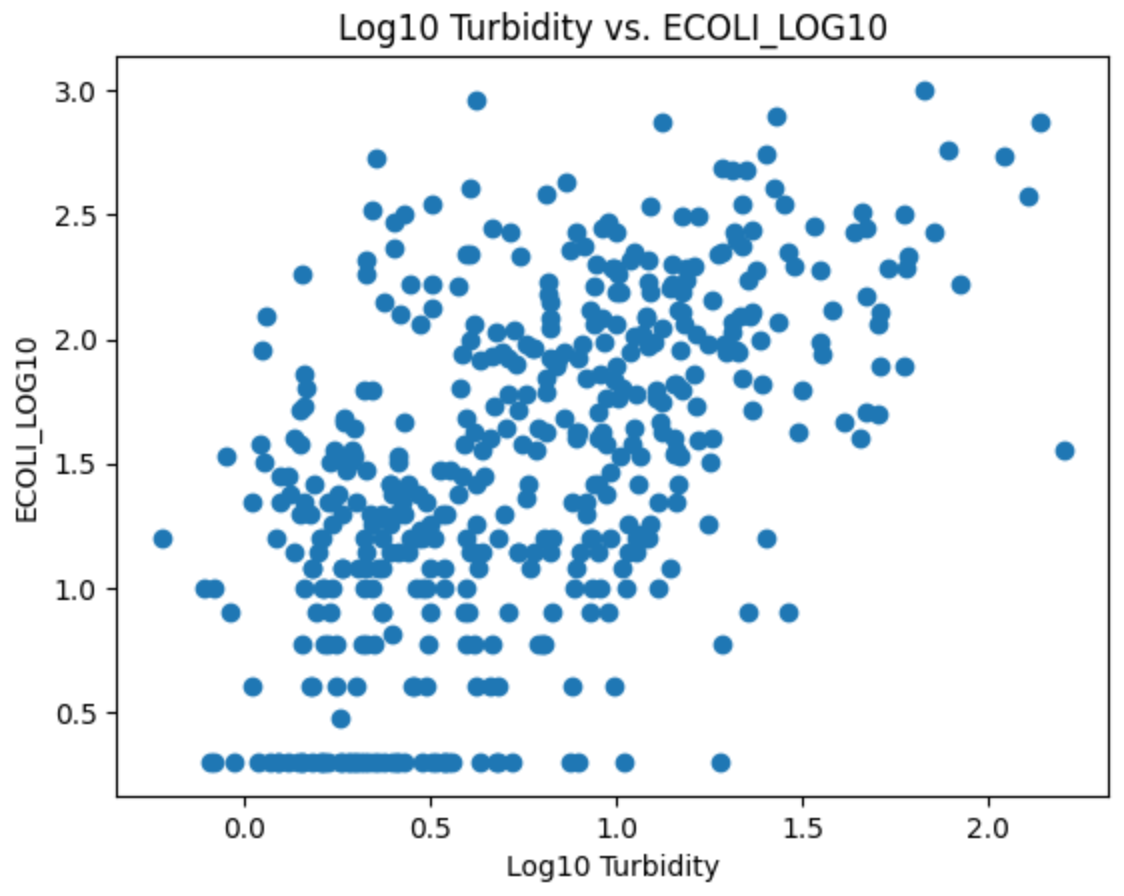
\includegraphics[width=0.47\textwidth]{figs/log10_turb_ecoli.png}
    \caption{Correlation between $\log_{10}$ turbidity and $\log_{10}$ $E. coli$ concentration.}
    \label{fig:turbecoli}
\end{figure}
\begin{figure}
    \centering
    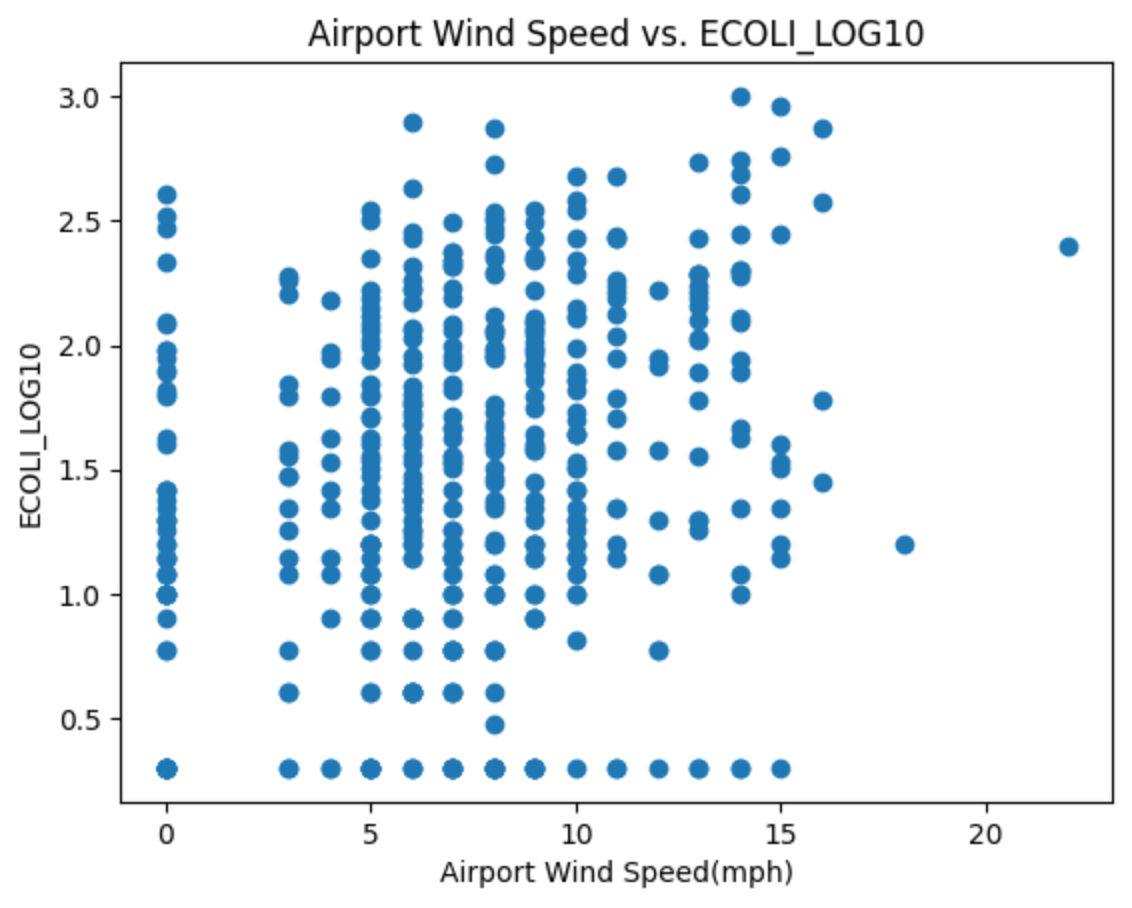
\includegraphics[width=0.47\textwidth]{figs/airportwindsp.png}
    \caption{Correlation between airport wind speed and $\log_{10}$ \textit{E. coli} concentration.}
    \label{fig:airportwindsp}
\end{figure}


\section{Experiments}
\label{sec:expts}

\subsection{Training Strategy \& Technique}
Both datasets were split using the 80-20 train/test split. Then we ran a 5-fold cross-validation on the training set only. We tuned the hyperparameters of the model with GridSearchCV. The hyperparameters we tuned were alpha for Ridge and Lasso models, the penalty, alpha, and l1-ratio for SGD models, and the degree and alpha for PolyRidge models. The hyperparameters that maximized CV R-squared were selected. This approach provides a low leakage estimate of generalization and guards against arbitrary hyperparameter selection. After selecting the best model using cross-validation, we refit it on the entire training set and evaluated it on the untouched test set, reporting R-squared and RMSE for an unbiased comparison with USGS baselines.

\subsection{Model 1: SGDRegressor}
Initially, we picked SGDRegressor as our first linear model to test. It uses the strategy of stochastic gradient descent to take each sample one at a time when measuring the gradient of loss. We set up using the L2 penalty by default to start with a maximum iteration of 1000.

\subsection{Model 2: Ridge}
We then switched from stochastic to batch-based models. This is because we wanted to see if the use of a batch-based model could produce a smoother convergence with a more accurate gradient. We first used ridge regression to serve as a direct comparison with stochastic gradient descent.

\subsection{Model 3: LASSO}
The purpose of trying LASSO was to test the change when switching from the L2 to the L1 penalty. We expect the model to generate coefficients that reflect the relevance of different parameters.

\subsection{Model 4: Polynomial Ridge}
We decided to move on from a linear regression model to a polynomial model because we wanted to explore what the performance would be if trained with higher-degree features. We used \texttt{PolynomialFeatures} from the \texttt{sklearn.preprocessing} to achieve it.

\subsection{Statistical Analysis}
We used the Python package \href{https://www.statsmodels.org/stable/index.html}{\texttt{statsmodels}} to help us assess the quality of our model. We did R-squared and p-value analysis to measure the fitness and accuracy of each coefficient of hyperparameters across different models.

\subsection{Differential Analysis}
We performed a differential analysis to sort out the top ten outliers with the greatest divergence between the predicted and actual values in our final coding files. We achieved this by pooling the predicted and actual values, calculating their differences, and sorting the absolute values in descending order. Eventually, we were able to generate a table of the top 10 outliers with their hyperparameter values.

\section{Results}
\label{sec:results}

Our final results and code are in \texttt{b6\_model\_final.ipynb} and \texttt{huntington\_model\_final.ipynb}. We evaluated the quality of fitting across all our models using the R-squared value and root mean square error (RMSE) analyses.
\subsection{Beach 6}
For the Beach 6 dataset, we found that all four models we generated have higher R-squared values while maintaining lower RMSE values than the published model (Figure \ref{fig:b6}). This result surprised us, although we realized that our fine-tuning of coefficients using cross-validation and grid search could contribute to better performance. Having lower scores on training data, yet higher scores on testing data, indicates the absence of overfitting in our models.\\
Looking into each model for the Beach 6 dataset, we found that the performance of Ridge and PolyRidge was the same. We then plotted the graphs of actual values versus predicted values for both models (Figure \ref{fig:b6ridge}, \ref{fig:b6poly}). We observed a consistent pattern of prediction versus actuality. This was due to the preference of hyper-parameter dimension by the grid search. We found that in our code, grid search selected degree = 1, which reduces to a linear model, leading to the identical performance by Ridge and PolyRidge.\\
The result of our differential analysis suggested that the prediction could be strongly affected by the hyperparameter \texttt{BIRDS\_NUM}. The huge swing between discrete numbers could potentially contribute huge variance during prediction. The p-value of the \texttt{BIRDS\_NUM} coefficient also suggested that, compared to other coefficients, it is more prone to generate variant results.
\subsection{Huntington}
For the Huntington dataset, our models generally performed as well as the published one (Figure \ref{fig:hunt}). The PolyRidge model wins with an exceptional $0.56590$ R-squared value and $0.4336$ RMSE. It indicates that the connections between hyperparameters are of significance to the prediction of \textit{E. coli} concentration in Huntington.\\
We also plotted the predicted versus actual values for the PolyRidge and Ridge models to see the differences. We observed that although the patterns are consistent when on the lower end ($\log_{10}$ \textit{E. coli} concentration $\leq 2.0$), the PolyRidge model produces more converged data on the higher end ($\log_{10}$ \textit{E. coli} concentration $> 2.0$). This suggested that in order to predict higher values better, a higher degree of hyperparameters is necessary.
The differential analysis unravels the effect of the hyperparameter \texttt{WaveHt\_Ft} on the prediction. We found multiple zero values among the top ten outliers. Since the model is using polynomial regression, any combination of hyperparameters associated with \texttt{WaveHt\_Ft} would be zero. This could cause a major fluctuation between the predicted and actual values.

\begin{figure}
    \centering
    \resizebox{0.47\textwidth}{!}{
        \begin{tabular}{|c|c|c|c|c|}
             \hline
             Model & Train $R^2$ Mean & Train RMSE Mean & Test $R^2$ & Test RMSE\\[3pt]
             \hline
             Published & N/A & N/A & $0.47697$ & $0.4841$\\[3pt]
             \hline
             Ridge & $0.42921$ & $0.5032$ & $0.48872$ & $0.4431$\\[3pt]
             \hline
             PolyRidge & $0.42921$ & $0.5032$ & $0.48872$ & $0.4431$\\[3pt]
             \hline
             SGD & $0.42833$ & $0.5029$ & $0.48851$ & $0.4432$\\[3pt]
             \hline
             LASSO & $0.42817$ & $0.5033$ & $0.48912$ & $0.4429$\\[3pt]
             \hline

        \end{tabular}
        }
    \caption{Model performance on the Beach 6 dataset}
    \label{fig:b6}
\end{figure}

\begin{figure}
    \centering
    \resizebox{0.47\textwidth}{!}{
        \begin{tabular}{|c|c|c|c|c|}
             \hline
             Model & Train $R^2$ Mean & Train RMSE Mean & Test $R^2$ & Test RMSE\\[3pt]
             \hline
             Published & N/A & N/A & $0.54985$ & $0.4432$\\[3pt]
             \hline
             PolyRidge & $0.54241$ & $0.4423$ & $0.56590$ & $0.4336$\\[3pt]
             \hline
             Ridge & $0.53913$ & $0.4438$ & $0.54807$ & $0.4424$\\[3pt]
             \hline
             LASSO & $0.53904$ & $0.4438$ & $0.54774$ & $0.4426$\\[3pt]
             \hline
             SGD & $0.53856$ & $0.4440$ & $0.54826$ & $0.4423$\\[3pt]
             \hline

        \end{tabular}
        }
    \caption{Model performance on the Huntington dataset}
    \label{fig:hunt}
\end{figure}

\begin{figure}
    \centering
    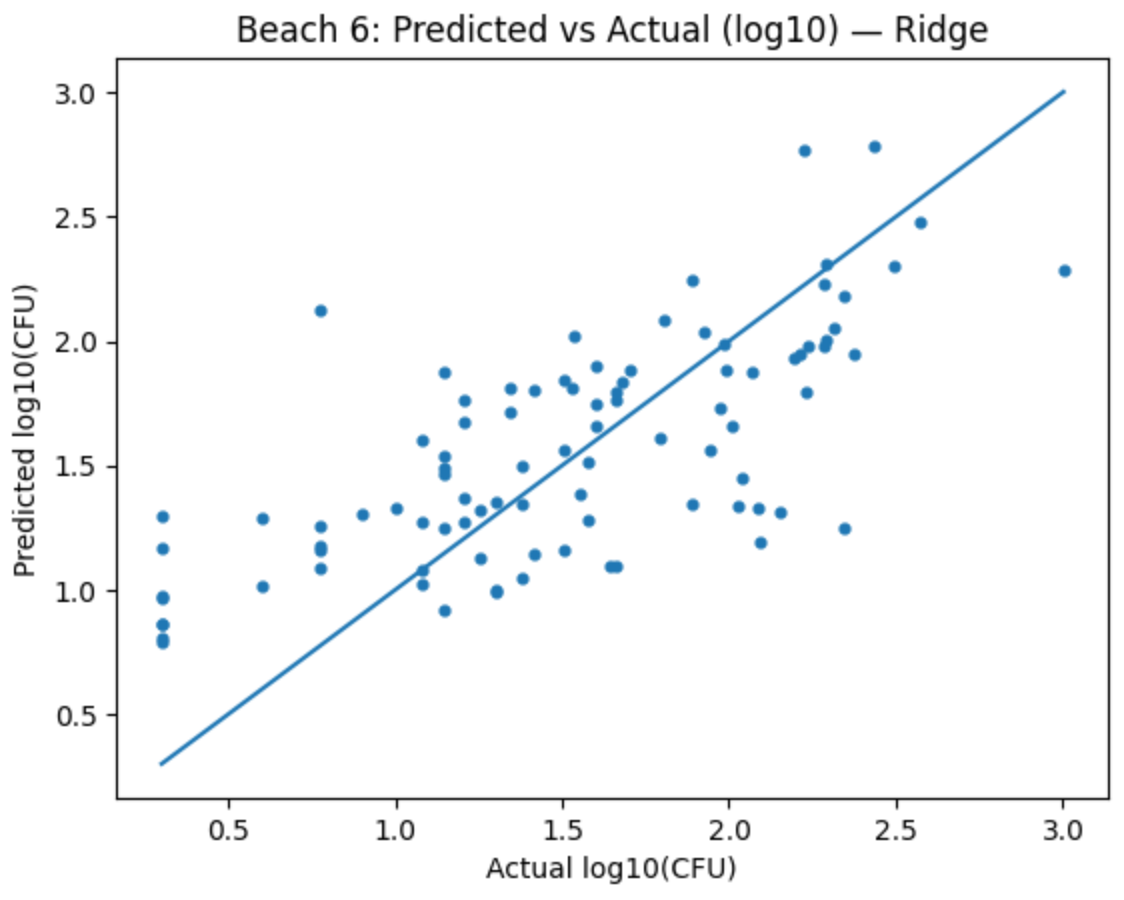
\includegraphics[width=0.86\linewidth]{figs/b6_ridge.png}
    \caption{Predicted versus actual values for Beach 6 dataset using Ridge linear regression model.}
    \label{fig:b6ridge}
\end{figure}

\begin{figure}
    \centering
    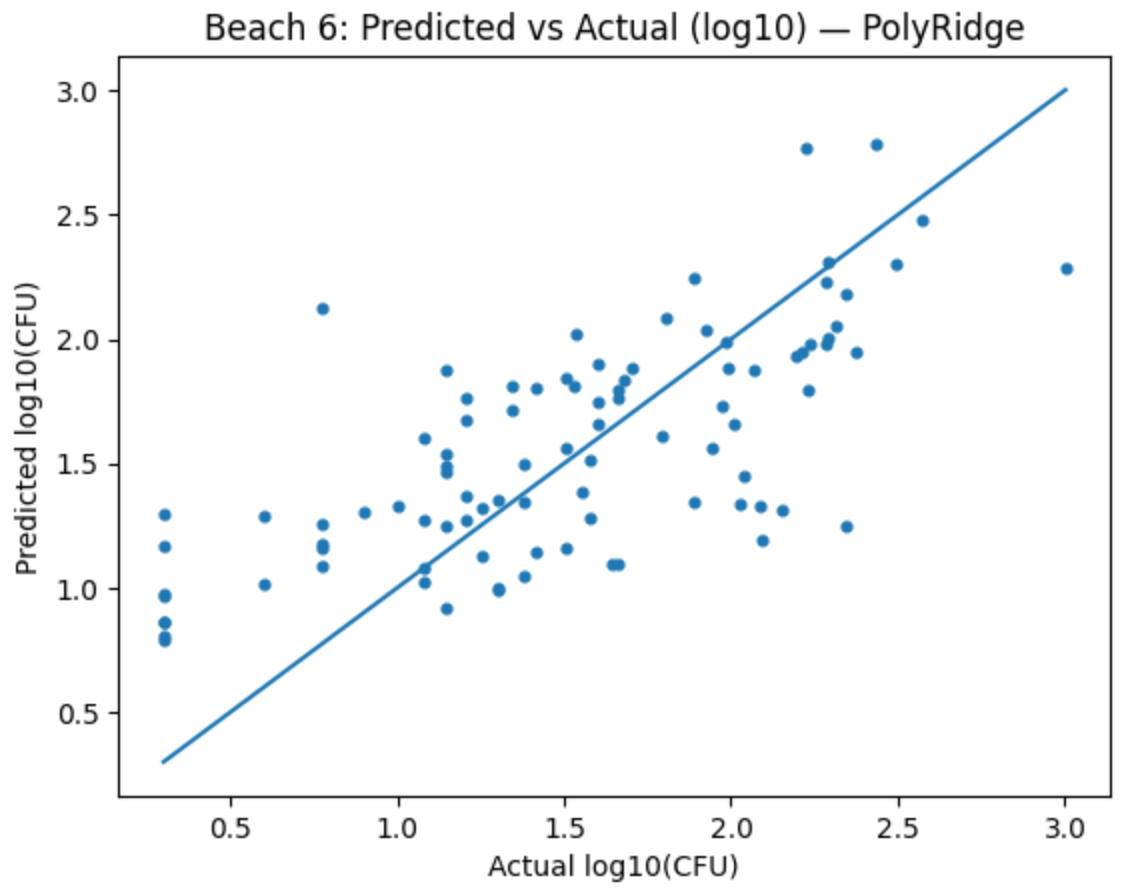
\includegraphics[width=0.86\linewidth]{figs/b6_poly.png}
    \caption{Predicted versus actual values for Beach 6 dataset using PolyRidge linear regression model.}
    \label{fig:b6poly}
\end{figure}

\begin{figure}
    \centering
    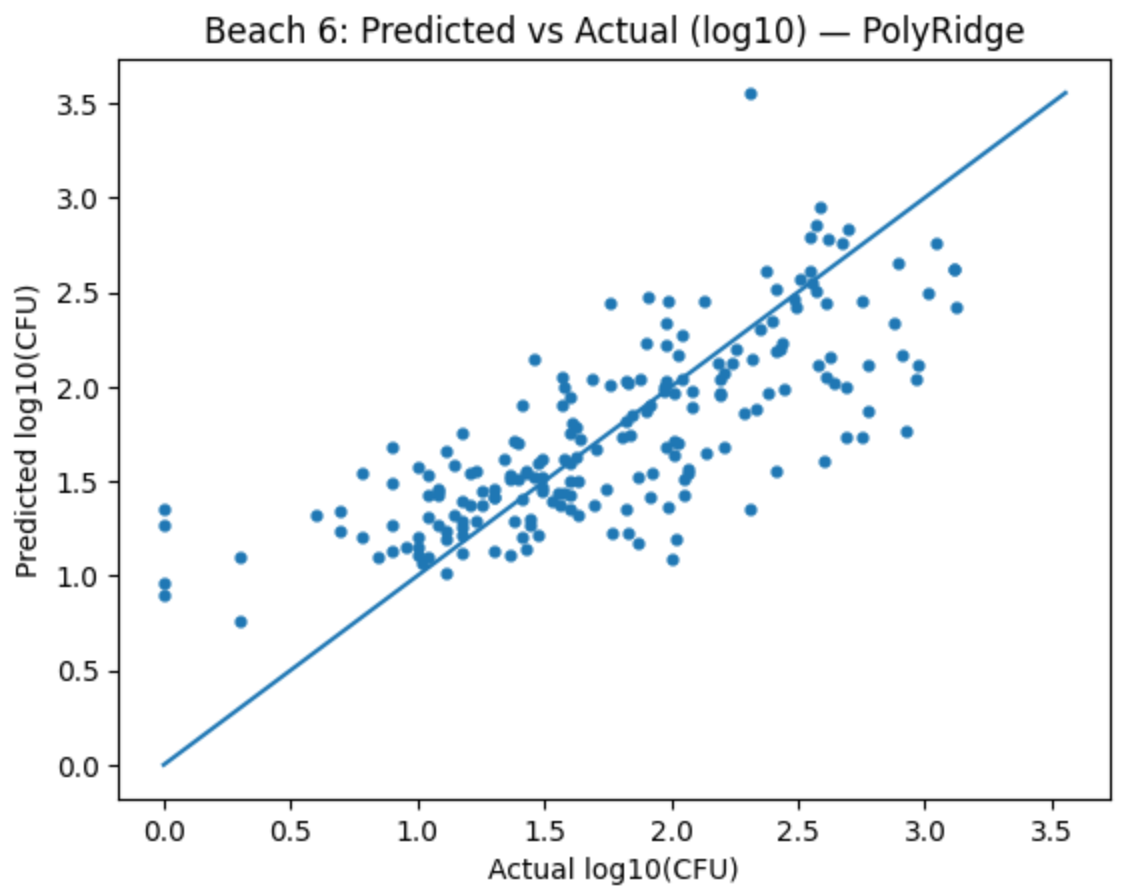
\includegraphics[width=0.86\linewidth]{figs/hunt_poly.png}
    \caption{Predicted versus actual values for Huntington dataset using PolyRidge linear regression model.}
    \label{fig:huntPoly}
\end{figure}

\begin{figure}
    \centering
    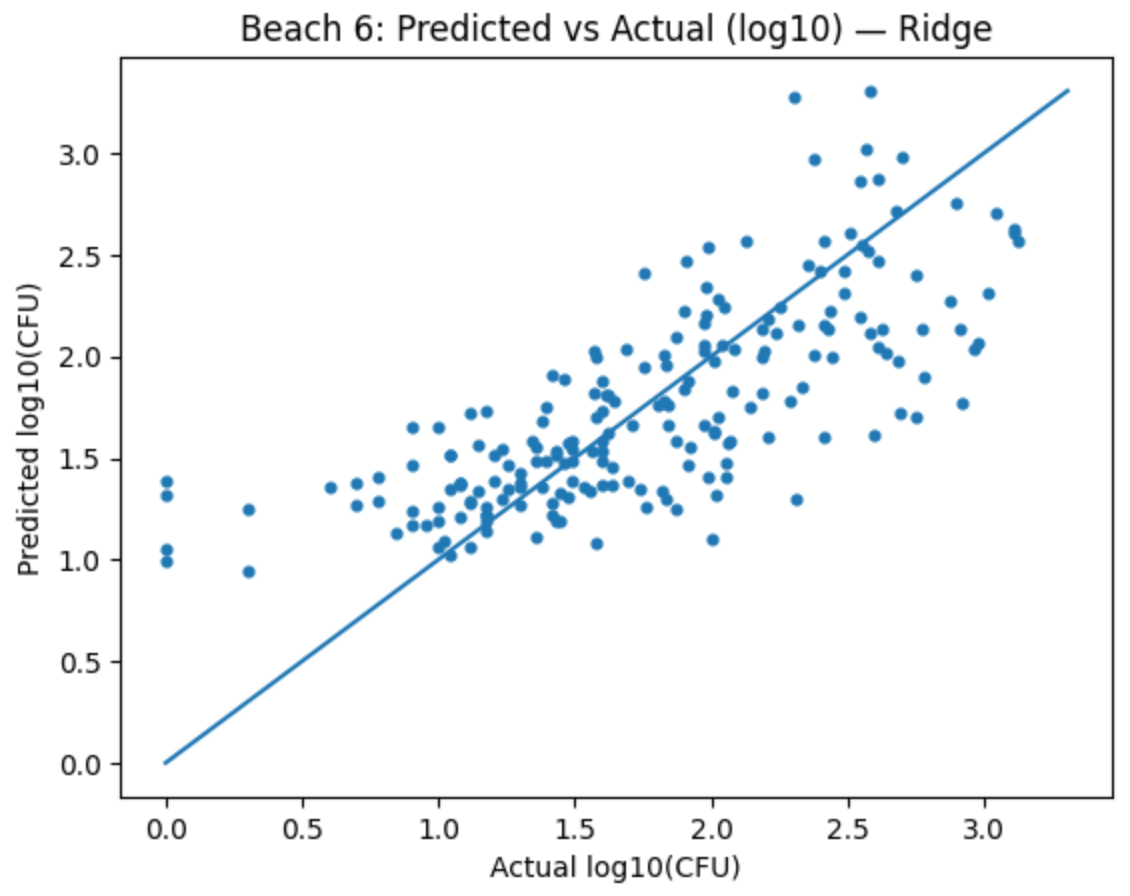
\includegraphics[width=0.86\linewidth]{figs/hunt_ridge.png}
    \caption{Predicted versus actual values for Huntington dataset using Ridge linear regression model.}
    \label{fig:huntRidge}
\end{figure}


\section{Broader Impacts}
\label{sec:impacts}

Our models predict the \textit{E. coli} concentration in water bodies from the Great Lakes region in Ohio and Pennsylvania. Based on data points related to such as water and weather conditions, we produced models that have similar or even better performances than the published model, indicating the possibility of generating better prediction using ours. However, a few concerns still remain in our mind at the end of this project.\\
The first concern is the generality of our model. Since the data was collected near two beaches that are considered as on-shore or near-shore areas, the models are limited by the data because it could only be applicable to similar environments. Furthermore, the prediction should not be reliable for predicting water quality in regions that are not similar as the Great Lakes region, which has a unique and complex system of environmental components. We believe that although the results of our models look good on the paper, the practicality of actual real-life use should be concerned before application.\\
The second is about the general data-driven prediction of water quality. We believe that it should be cautious to take experimental models into real-life applications. Using data-driven model for water quality prediction could potentially cause major public health issues if done wrong. As mentioned above, the limitation of both our models and the published one is obvious and should be used with caution when used in real life. One way to make the models more applicable is to limit the scope: for example, concentrating on predicting water quality in agricultural pond water \cite{Stocker}. By limiting the prediction target, models could be more reliable when used for the specific scenario when data collection were standardized ideally. 

\section{Conclusions}
\label{sec:concl}

Our work produces two regression models using machine learning that predict water quality in water bodies around the Great Lakes region. For the Beach 6 dataset, we found that the linear regression model using Ridge produces the most statistically successful result. For the Huntington data, the polynomial regression using Ridge generates a better prediction, as it deals with the interconnected relationships among hyperparameters. We believe that our models could be useful for progressing the water-quality machine learning model for Great Lakes region but should be used with caution when dealing with other more generalized environments. One potential future direction could be standardizing the data collection of water bodies across the Great Lakes region to produce a more generalized model with a wider scope.

\section{Contributions}
\label{sec:contrib}
Both B.C. and R.W. did the early exploration and the pre-processing of the data. B.C. experimented with the first few models on the Beach 6 dataset. R.W. experimented with the Huntington dataset for the similar models. B.C. experimented cross-validation and grid search for coefficient tuning and integrated the models together for statistical analyses. R.W. was responsible for writing the textual part of the write-up. Both contributed in making figures and tables. Both have proofread and made final editing of the document upon submission. 



% This creates the references section. Open the project1.bib file to
% see how to organize your references.
\bibliography{project1}
\bibliographystyle{aaai} % sets citation and bib style, do not modify

\end{document}
